\startchapter{Analysis Preparation}
\label{chapter:ana_prep}

\section{Signal Model}
This work concerns a search for dark matter produced in association with a dark Higgs boson as described in subsection \ref{subsection:dh_model}.  The dark Higgs boson, $s$, then decays to standard model particles with the same branching ratios as a standard model Higgs boson of variable mass, as shown in Figure \ref{fig:HiggsBR}. At low $s$ mass, this is dominated by a decay to a pair of $b$ quarks, and is currently being studied via a reinterpretation of the ATLAS search for dark matter produced in association with a standard model Higgs boson decaying to $b\bar{b}$ in \cite{monos_bb}. At $s$ masses above 160 GeV, however, the decay to a pair of $W$ bosons, shown in Figure \ref{fig:dh_feynman}, becomes kinematically available on-shell. Even slightly below this threshold, $s$ decays to $WW$ are the dominant process. The pair of $W$ bosons decay rapidly, and are not detected as final state particles by the ATLAS detector. Instead, they each decay either to hadronic ($q\bar{q}$) or leptonic ($l\nu$) final states. A search in the fully hadronic channel, with both $W$ decaying to $q\bar{q}$, is complete (see \cite{had_analy}), and this work focuses on the semileptonic decay channel with one $ W \rightarrow q\bar{q} $ and one $ W \rightarrow l\nu $. When both analyses are complete, the results will be statistically combined.

\begin{figure}[H]
    \centering
    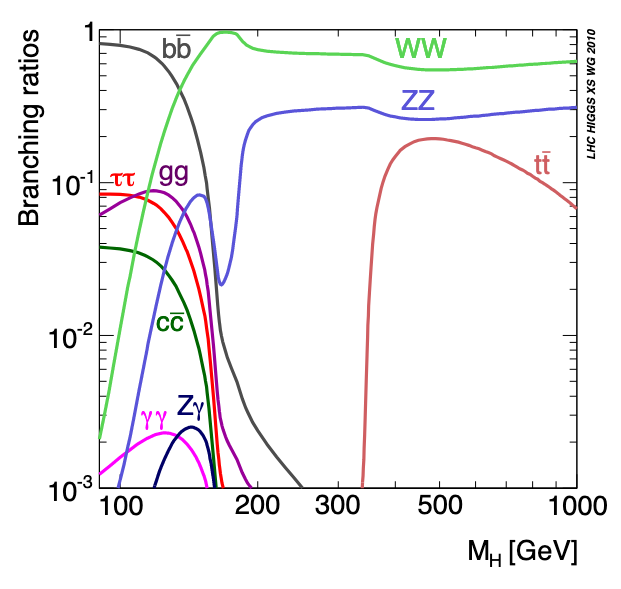
\includegraphics[width=0.8\textwidth]{Figures/3/HiggsBR.png}
    \caption{Branching fractions for a SM Higgs boson as a function of the Higgs boson mass \cite{Higgs_BR}.}
    \label{fig:HiggsBR}
\end{figure}

\begin{figure}[H]
    \centering
    \feynmandiagram [horizontal=a to b] {
    i1[particle=\(q\)] -- [fermion] a -- [fermion] i2[particle=\(q\)],
    a -- [boson, edge label=\(Z'\)] b,
    b -- [boson, edge label=\(Z'\)] c,
    b -- [scalar, edge label=\(s\)] d,
    f1[particle=\(\chi\)] -- [fermion] c -- [fermion] f2[particle=\(\chi\)],
    f3[particle=\(W\)] -- [boson] d -- [boson] f4[particle=\(W\)],
    f2 -- [opacity=0.0] f3
    };
    \caption{Dark Higgs boson decay}
    \label{fig:dh_feynman}
\end{figure}

In the ATLAS detector, this signal signature will be characterized by a single lepton in the final state from the $ W \rightarrow l\nu $ decay, along with a pair of jets from the $ W \rightarrow q\bar{q} $ decay and a strong missing transverse momentum signature from the dark matter particles and neutrino.

\section{Monte Carlo Production and Data}
\label{section:mc_prod}
In order to search for a signal such as the one described above, it is necessary to form a prediction which can be compared with data from the ATLAS detector. In order to achieve this, simulated data is produced using Monte Carlo (MC) generators according to standard model predictions. This represents ``background" data, or what we would expect to see if the signal process did not exist. Added to this, signal MC samples are produced according to the signal model. Then, after isolating for an area of phase space that would be rich in signal events, the ATLAS data can be compared with the simulated data with or without signal events to make statistical conclusions about the likelihood of the existence. The following sections will detail the MC and data samples prouduced for ths analysis.

\subsection{Signal MC}
\label{subsection:mc_signal}
Signal samples are produced using the model and parameter choices outlined in subsection \ref{subsection:dh_model}. They are produced by calculating the hard process cross-section at leading order (LO) using \mgamc 2.7.2 \cite{MadGraph} interfaced with \pythia 8.230 \cite{Pythia} for parton shower modelling. The CKKW-L \cite{CKKW} procedure with a matching scale of min($\frac{m_s}{4}$, $40~\text{GeV}$) is used to prevent overlap between the cross-section matrix element and parton shower. Two separate signal grids were produced, with the second covering an expanded parameter space. In the first, \mgamc is used with the NNPDF30 LO PDF set with $\alpha_s = 0.13$ \cite{PDF30}, while in the second \mgamc is used with the NNPDF30 NLO PDF set with $\alpha_s = 0.118$ \cite{PDF30}. The signals studied span a parameter space in \ms and \mZp with samples produced at the mass points shown in Figure \ref{fig:signal_grid}.

\begin{figure}[H]
    \centering
    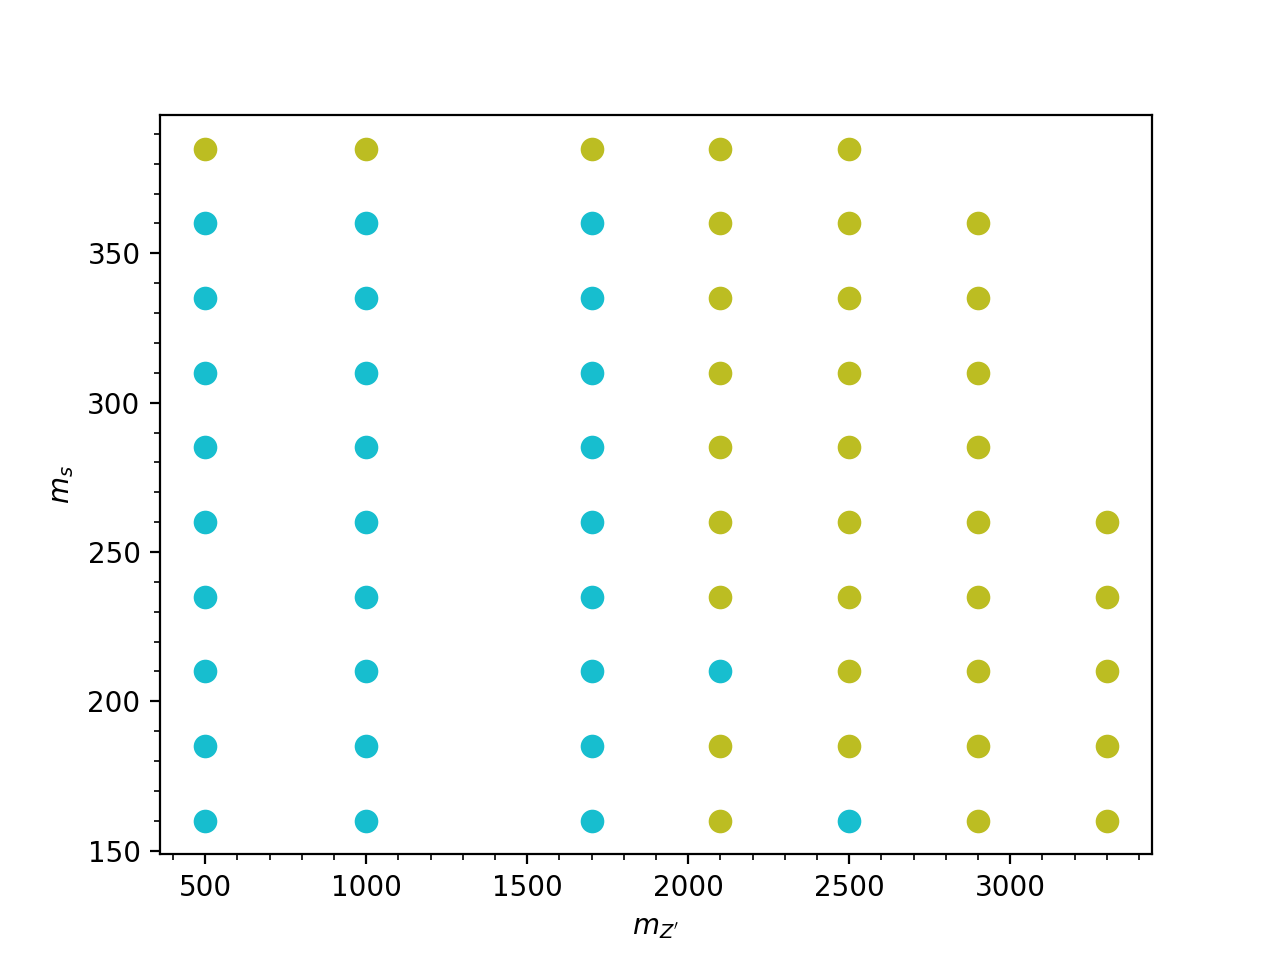
\includegraphics[width=0.8\textwidth]{Figures/3/SignalGrid.png}
    \caption{Signal point locations in \ms vs.~\mZp parameter space. Blue points represent the original signal grid, while green points are added in the second signal grid.}
    \label{fig:signal_grid}
\end{figure}

\subsection{Background MC}
\label{subsection:mc_bkg}
The dominant and sub-dominant SM backgrounds for this analysis are:
\begin{itemize}
    \item \wjets events, containing a single $W$ boson and 1 or more jets,
    \item \ttbar, containing with a top and anti-top pair, and
    \item di-boson events, containing a pair of vector bosons.
\end{itemize}
Additionally, \zjets, tri-boson, and single-top quark\footnote{In some plots in this work single-top quark events are denoted by the short form ``stop". This is not to be confused with a supersymmetric partner of a top-quark often referred to as a ``stop".} events make non-negligible background contributions. All background contributions are estimated using MC simulated data, and the \wjets and \ttbar backgrounds are further constrained using data-driven control regions.

\subsubsection{\vjets, Di-boson, and Tri-boson}
Two distinct sets of \wjets and \zjets (\vjets) background samples are used. The samples are simulated with the \sherpa v2.2 MC generator \cite{Sherpa} with up to two additional parton emissions at NLO or four additional parton emissions at LO accuracy \cite{VJets}\cite{VJets_mW}. Merging of parton showers with matrix elements is achieved using CKKW \cite{CKKW} matching with the MEPS@NLO prescription extending this to NLO \cite{MEPS}. The NNPDF30 NNLO PDF set is used \cite{PDF30}.

The difference between these two sets of samples is that first set is produced using \sherpa v2.2.1, and the second with \sherpa v2.2.10. As well, additional statistics-enhanced \wjets samples are added to the second set with $m_W > 120$ GeV \cite{VJets_mW}. This greatly increases the number of simulated events in this small section of phase space that is important to this analysis. Overlap removal in $m_W$ is performed between these mass-enhanced samples and the other \wjets samples.

Di-boson and tri-boson samples are similarly generated with only a single set using either \sherpa v2.2.1 or v2.2.2 depending on the process, and CKKW matching is again used to merge parton shower and matrix element simulation.

\subsubsection{\ttbar and single-top}
MC samples for the \ttbar and single-top standard model background process are modelled using the \powhegbox v2 \cite{Powheg} generator, which gives matrix elements at NLO in the strong coupling constant $\alpha_s$. This uses the NNPDF30 NLO PDF set \cite{PDF30}. Similar to the signal samples, this is combined with \pythia 8.230 \cite{Pythia} for parton shower modelling using the NNPDF23 LO PDF set \cite{PDF23}.

\subsection{Data}
This analysis uses data from the full Run-2 period, i.e. from 2015-2018, with individual runs selected using the good runs lists:
{ \scriptsize
\begin{itemize}
	\item \GRLa
	\item \GRLb
	\item \GRLc
	\item \GRLd
\end{itemize}
}
This results in a total integrated luminosity of 138.5 fb$^{-1}$.

\subsubsection{MC Scaling to Match Data Luminosity}
\label{subsubsection:mc_scaling}
The events in MC simulated samples above must be re-weighted in order to match the total integrated luminosity of the ATLAS data used. In order to achieve this, the weight of each MC event is given by:
\begin{equation}
\text{weight}  = \frac{ \sigma \times (138.5~\text{fb}^{-1}) \times (k) \times (\text{filt}_\text{eff}) \times (\text{GenWeight}) \times (w_f)}{\sum_{\text{Events~in~AOD}} \text{GenWeight} }
\end{equation}
where
\begin{itemize}
\item \sigma~is the cross section for the simulated process in fb,
\item $k$ is the k-factor, which corrects for the omission of higher-order terms in event generation,
\item $\text{filt}_\text{eff}$ is the filter efficiency, the fraction of events passing any filters applied during event generation to emphasize a certain phase space,
\item GenWeight is the generator weight from MC production,
\item and $w_f$ is a set of weight factors given by:
\begin{equation}
w_f = \text{EleWt} \times \text{MuoWt} \times \text{JetWtJVT} \times \text{prwWt}
 \times \text{TriggerWts}
\end{equation}
where the various weights apply small corrections from the generation and reconstruction process.
\end{itemize}


\section{Object Definition}
\label{section:objects}
Once events have been simulated or produced in the ATLAS detector, the information contained in them must be reconstructed into objects which can be analyzed. These objects represent particles or groups of particles, and are used to fully or partially reconstruct events and search for signal signatures. The following section will detail the definition of physics objects used in this analysis.

\subsection{Muons}
\label{subsection:muons}
From the ATLAS detector, muons are reconstructed from measurements in the Inner Detector and the Muon Spectrometer. For this analysis, two different definitions of muon candidates are used. ``\textit{Baseline}" muons use slightly looser selection criteria than ``\textit{signal}" muons, which are designed for high purity. \textit{Baseline} muons are selected using the \textit{Loose} identification criteria as defined in \cite{muon_wp}, which is designed to maximize efficiency. \textit{Signal} muons, meanwhile, use the \textit{Medium} identification criteria, and must also be isolated from other signatures according to the \textit{Tight} track-based working point, with variable radius dependent on \pT. Additionally, all muons are rejected if they are considered ``badly reconstructed" or ``cosmic", and track-to-vertex association cuts are applied. Table \ref{tab:muon_criteria} summarizes the muon selection criteria.

\begin{table}[H]
\centering
\caption{Muon object definition criteria}
\label{tab:muon_criteria}
\begin{tabular}{l l l}
\toprule
\textbf{Criterion} & \textbf{Baseline Muon} & \textbf{Signal Muon} \\
\midrule
Identification & \verb|Loose| & \verb|Medium| \\
Isolation & - & \verb|TightTrackOnly_VarRad| \\
\midrule
Pseudorapidity & \(\abs{\eta} < 2.7\) & \(\abs{\eta} < 2.5\) \\
\pT & \(\pT > \unit[7]{\GeV} \) & \(\pT> \unit[7]{\GeV} \) \\
\midrule
Veto & Cosmic or Bad & Cosmic or Bad \\
\midrule
\multirow{2}{*}{Track-to-vertex association} & \(\abs{d_0 / \sigma_{d_0}}  < 3 \) & \( \abs{d_0 / \sigma_{d_0}}  < 3 \) \\
	& \( \abs{\Delta z_0^\textrm{BL} \sin \theta} < \unit[0.5]{mm} \) & \( \abs{\Delta z_0^\textrm{BL} \sin \theta} < \unit[0.5]{mm} \) \\
\bottomrule
\end{tabular}
\end{table}

\subsection{Electrons}
\label{subsection:electrons}
Electrons are reconstructed by associating energy deposits in the EM calorimeter with tracks in the inner detector. Similar to muon candidates, two different definitions are used, with ``\textit{baseline}" electrons requiring slightly less selective criteria than ``\textit{signal}" electrons. \textit{Baseline} and \textit{signal} electrons are selected using a likelihood-based identification described in \cite{e_wp}. \textit{Signal} electrons require the medium identification criteria, while \textit{baseline} electrons requre the loose criteria as well as a hit in the innermost layer of the pixel detector. Additionally, \textit{baseline} and \textit{signal} electrons must both satisfy the fixed-cut \textit{Loose} isolation requirement. Like for muons, track-to-vertex association cuts are also applied. Table \ref{tab:electron_criteria} summarizes the electron selection criteria.

\begin{table}[H]
\centering
\caption{Electron object definition criteria}
\label{tab:electron_criteria}
\begin{tabular}{l l l}
\toprule
\textbf{Criterion} & \textbf{Baseline Electron} & \textbf{Signal Electron} \\
\midrule
Identification & \verb|LooseAndBLayerLLH| & \verb|MediumLLH| \\
Isolation & \verb|FCLoose| & \verb|FCLoose| \\
\midrule
Pseudorapidity & \(\abs{\eta} < 2.47\) & \(\abs{\eta} < 2.47\) \\
\pT & \(\pT > \unit[7]{\GeV} \) & \(\pT> \unit[7]{\GeV} \) \\
\midrule
\multirow{2}{*}{Track-to-vertex association} & \(\abs{d_0 / \sigma_{d_0}}  < 5 \) & \( \abs{d_0 / \sigma_{d_0}}  < 5 \) \\
	& \( \abs{\Delta z_0^\textrm{BL} \sin \theta} < \unit[0.5]{mm} \) & \( \abs{\Delta z_0^\textrm{BL} \sin \theta} < \unit[0.5]{mm} \) \\
\bottomrule
\end{tabular}
\end{table}

\subsection{Small-radius ($R=0.4$) Jets}
In this analysis, small-$R$ jets are used to reconstruct the hadronically-decaying $W$ boson in some analysis regions. Small-$R$ jets are reconstructed using particle-flow objects \cite{PFlow} clustered with the \akt algorithm \cite{antikt} with radius $R=0.4$. A jet of radius $R$ falls within a cone satisfying:
\begin{equation}
\Delta R(\text{axis}, \text{slant}) = R
\end{equation}
where $\Delta R$ between two points is given by:
\begin{equation}
\Delta R = \sqrt{\Delta\eta^2+\Delta\phi^2}
\end{equation}
with $\phi$ denoting the azimuthal angle about the beam axis, and $\eta$ denoting the pseudorapidity given by $\eta = -\ln[\tan(\frac{theta}{2})]$ where $\theta$ is the angle from the beam axis. Following reconstruction, only jets with $\pT > 20$ GeV and $|\eta| < 2.5$ GeV are used for analysis. Additionally, in order to suppress noise from pileup, the jet vertex tagger \cite{JVT} is applied with the \verb|Tight| working point.

\subsubsection{$b$-jets}
For this analysis, it is also beneficial to identify jets originating from bottom ($b$) quarks. In signal regions these jets are vetoed to reduce background. This is performed using the \verb|DL1r| \cite{DL1r} $b$-tagging algorithm, which employs a deep-learning neural network. A 77\% efficient tagger working point is used. Table \ref{tab:r04_criteria} summarizes $R=0.4$ jet criteria and tagging.

\begin{table}[H]
\centering
\caption{$R=0.4$ jets object definition criteria}
\label{tab:r04_criteria}
\begin{tabular}{l l}
\toprule
\textbf{Criterion} & \textbf{Requirement} \\
\midrule
Collection & \verb|AntiKt4EMPFlowJets| \\
\midrule
Pseudorapidity & \(\abs{\eta} < 2.5\) \\
\pT & \(\pT > \unit[20]{\GeV} \) \\
\midrule
Jet-Vertex-Tagger WP & \verb|Tight| \\
\midrule
$b$-tagger & \verb|DL1r| \\
\bottomrule
\end{tabular}
\end{table}

\subsection{Track-Assisted-Reclustered Jets}
\label{ap:TARjet_object_defs}
Track-Assisted-Reclustered (TAR) jets \cite{TAR} are used in this analysis to reconstruct hadronically-decaying $W$ boson candidates in some regions. $R=0.2$ jets, constructed with the \akt algorithm \cite{antikt} from locally-calibrated topological clusters \cite{TopoClusters} are used as input for building TAR Jets. As well, the TAR algorithm uses tracks fulfilling quality criteria outlined in Table \ref{tab:TARparameters}. The TAR building process involves constructing large-$R$ jets from the constituent small-$R$ jets. Tracks are then matched with the input jets and rescaled using the $p_T$ of the matched jets. The kinematic properties of the TAR jets are then calculated from the constituent $R=0.2$ jets, while the jet substructure variables are calculated from the constituent tracks. Figure \ref{fig:TAR_alg} shows a visual summary of the base TAR algorithm, and
the following steps outline the algorithm in more detail:
\begin{itemize}
  \item Tracks and calibrated \akt $R=0.2$ jets are chosen as input to the algorithm.
  \item The \akt $R=0.2$ jets are reclustered using the \akt algorithm into $R=1.0$ jets and trimmed using the $p_T$ fraction \(f_{cut}=0.05\).
  \item Input tracks are matched to $R=0.2$ jets, if possible, using ghost association \cite{Ghost}.
  \item Tracks which remain unassociated are matched to the nearest \akt $R=0.2$ jet within $\Delta R<0.3$
  \item The \pT of each track is rescaled using the \pT of the jet to which it is matched, via the equation:
  \begin{equation}
  \pT^{\text{track, new}} = \pT^{\text{track, old}}\times \frac{\pT^{\text{subjet $j$}}}{\sum_{i \in j} \pT^{\text{track $i$}}} ,
  \label{eq:TAR_rescale}
  \end{equation}  where $j$ is the $R=0.2$ subjet that the track being rescaled is matched with, and the index $i$ runs over all tracks matched to that subjet. This rescaling accounts for the missing neutral momentum, which is measured at calorimeter level but is not present at tracker level.
  \item Finally, jet substructure variables and $m^\text{TAR}$ are calculated using the rescaled matched tracks.
\end{itemize}
The parameters of the TAR algorithm used are summarized in Table \ref{tab:TARparameters}. \\

\begin{table}[H]
\centering
\caption{TAR jet reconstruction parameters}
\label{tab:TARparameters}
\begin{tabular}{l l }
\toprule
\multirow{3}{*}{Input track selection} & \verb|Loose| quality\\
	& \(\pT > 0.5~\GeV\) \\
	& \(\abs{\eta} < 2.5\)  \\
  \multirow{2}{*}{Track-to-vertex association} & \(\abs{d_0}  < \unit[2]{mm} \) \\
  	& \( \abs{\Delta z_0^\textrm{BL} \sin \theta} < \unit[3.0]{mm} \) \\
\midrule
\multirow{3}{*}{Input jet selection} & $R=0.2$ topo jets \\
	& \(\pT > 20~\GeV\) \\
	&  \(\abs{\eta} < 2.5\)  \\
\midrule
Reclustering radius & \(R=1.0\) \\
TAR jet \pT & \(\pT^\text{TAR} > 100~\GeV\) \\
Trimming radius & \(R=0.2\) \\
Trimming \pT fraction & \(f_\text{cut}=0.05\) \\
Track-to-jet association & \(\Delta R(\text{jet, track}) < 0.3\) \\
\bottomrule
\end{tabular}
\end{table}

\begin{figure}[H]
    \centering
    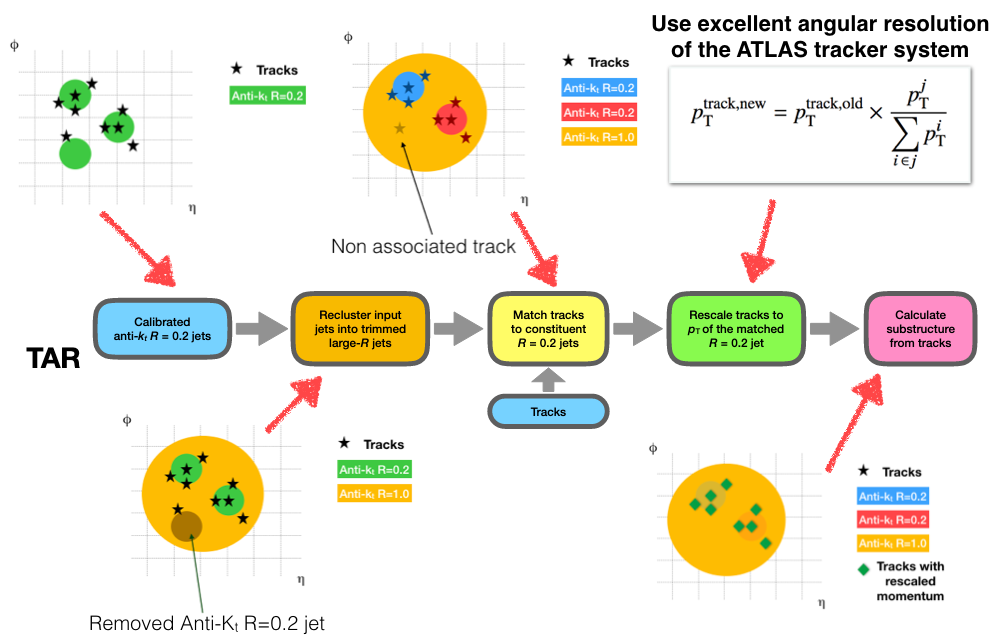
\includegraphics[width=0.9\textwidth]{Figures/3/TAR_alg.png}
    \caption{A visual summary of the TAR Jet algorithm. \cite{TAR_image}}
    \label{fig:TAR_alg}
\end{figure}

\subsection{Missing Transverse Momentum (\met)}
In the ATLAS detector, the beams collide directly along the longitudinal axis. As a result of the conservation of momentum, all decay products from the collision should thus have a total transverse momentum of 0. Using this information, missing transverse momentum (\met) can be used to represent undetected objects. In the signal model described in subsection \ref{subsection:dh_model} both the neutrino from the leptonically decaying $W$-boson and the dark matter would not be directly detected in ATLAS. It is impossible to disentangle these objects, and they are reconstructed together using \met. \met is calculated for this analysis using baseline electrons and muons as described in subsections \ref{subsection:electrons} and \ref{subsection:muons}, as well as $R=0.4$ jets with the \verb|Tight| working point applied. No photons or \tau-leptons are included in the calculation. An additional soft term, which is calculated from tracks not associated with the reconstructed objects, is also added.

\subsubsection{\met Significance}
The significance of the \met measurement is also assessed using the object-based \met significance \metsig. It is calculated as described in \cite{MetSig} from a combination of the uncertainties on the reconstructed objects and soft term used to calculate \met, as well as a pileup correction. A high \metsig indicates a higher degree of confidence that the \met measurement of an event comes from an unseen object rather than from particle mismeasurement.

\section{Data and MC Preparation}
After reconstruction (or simulated reconstruction) in the ATLAS detector, data and MC events are stored as Analysis Object Data (AOD) files which contain all reconstructed information from each event. Data and MC samples used for this analysis are initially in ATLAS Derived Analysis Object Data (DAOD format) which are created by skimming and slimming the AODs according to the EXOT27 job options in the Athena framework \cite{Athena}. The DAODs include information about:
\begin{itemize}
	\item electrons, photons, muons, tau jets,
	\item $R=1.0$ jets,
	\item AntiKt4EMTopoJets, AntiKt4EMPFlowJets, AntiKt2LCTopoJets,
  \item jet b-tagging, and
	\item InDetTrackParticles associated with TopoJets
\end{itemize}

The DAOD files are still too large to be convenient for analysis, and some analysis variables have not yet been calculated. In order to further process the DAODs we use the XAMPP analysis framework, which is built on top of the SUSYTools framework within Athena. We use a customized version of the XAMPP framework (XAMPPMonoSlep) maintained by the analysis team to calculate all necessary analysis variables and selects physics objects according to the definitions in Section \ref{section:objects}. We used the following set of ``preselection" criteria to trim the number of events to a convenient size prior to optimization, without cutting into any regions of sensitivity:
\begin{itemize}
\item passed \met trigger,
\item (1 signal muon or 1 signal electron) and no additional baseline muons or electrons,
\item \met > 150 \GeV,
\item \metsig > 5,
\item transverse mass of \met and lepton \mtlepmet > 50 \GeV,
\item veto on $b$-tagged $R=0.4$ jets, and
\item \(\NTAR > 0\) or \(\Njets > 1\).
\end{itemize}

The trigger requirements beyond the preselection criteria are discussed in further detail in Section \ref{section:trig}.  After processing by the XAMPPMonoSlep framework, the data is stored in CERN ROOT files known as ``ntuples", which are further slimmed to include only necessary variables using XAMPPPlotting. At this stage the data and MC samples are ready to be analyzed.
